\subsection{Distribution -- System architecture}
As we previously said, our system is a simulator whose computation spreads
across multiple nodes.

We thought it was reasonable to divide our system in four subsystems, in order
to reason more easily about it. An overall view of our architecture is depicted
in Figure \ref{fig:sd-sys-arch-overall}:

\begin{figure}[H]
  \centering
  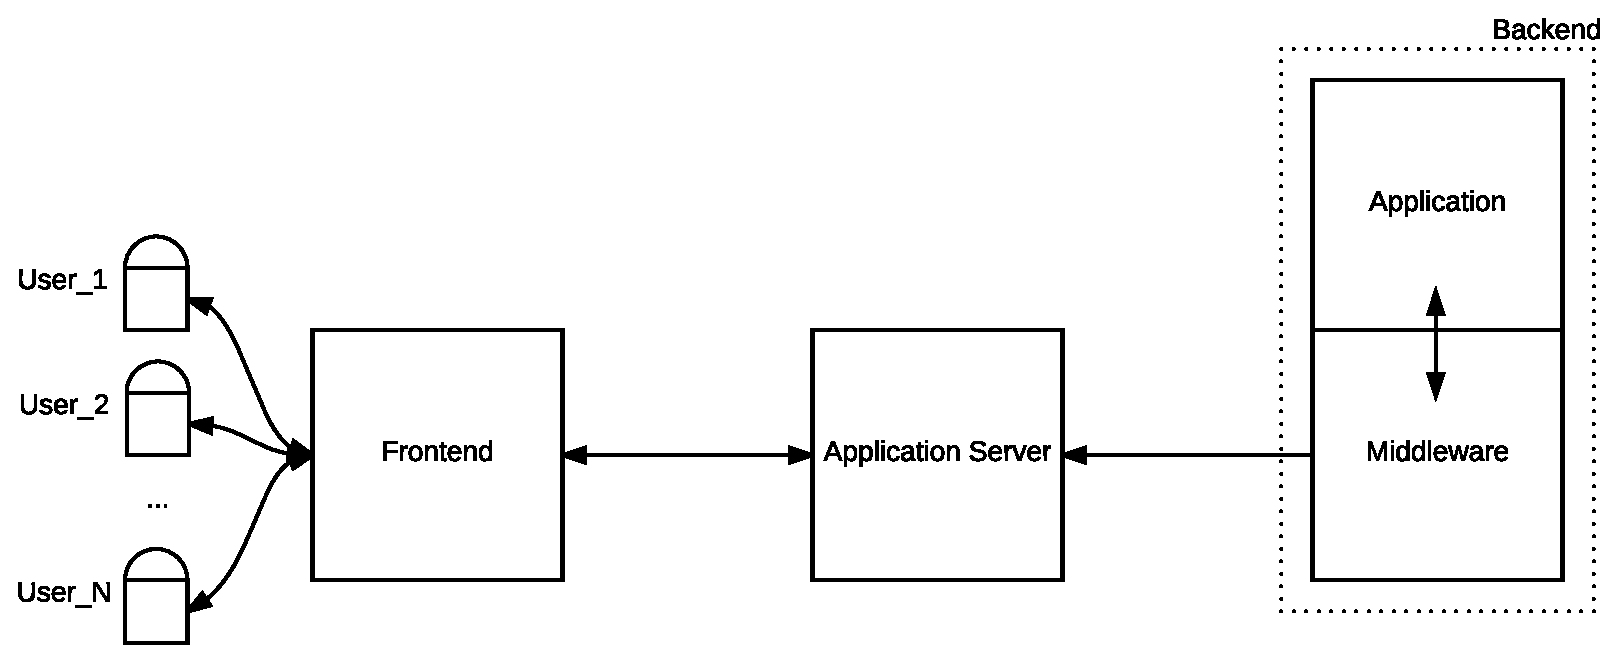
\includegraphics[scale=0.5,keepaspectratio]
    {images/solution/overall-arch.eps}
  \caption{Overall system architecture}
  \label{fig:sd-sys-arch-overall}
\end{figure}

As we can see from Figure \ref{fig:sd-sys-arch-overall}, we have:

\begin{itemize}
  \item a \textbf{Backend}, composed by the \textbf{Application} and the
    \textbf{Middleware} layers;
  \item the \textbf{Application Server}, which is responsible of handling
    information that arrives from the backend and to serve it to the frontend;
  \item a \textbf{Frontend}, which offers streaming services to end users.
\end{itemize}
